\documentclass[sigconf]{acmart}
\usepackage{booktabs}
\usepackage[dvipsnames]{xcolor}


%% \BibTeX command to typeset BibTeX logo in the docs
\AtBeginDocument{%
  \providecommand\BibTeX{{%
    \normalfont B\kern-0.5em{\scshape i\kern-0.25em b}\kern-0.8em\TeX}}}

%% These commands are for a PROCEEDINGS abstract or paper.
\settopmatter{printacmref=false} % Removes citation information below abstract
\renewcommand\footnotetextcopyrightpermission[1]{} % removes footnote with conference information in 

\acmConference[AEPRO 2024]{AEPRO 2024: Algorithm Engineering Projects}{March 1}{Jena, Germany}

% convert text to title case
% http://individed.com/code/to-title-case/

% that helps you to formulate your sentences
% https://www.deepl.com/translator

\begin{document}

%%
%% The "title" command has an optional parameter,
%% allowing the author to define a "short title" to be used in page headers.
\title[Project 1: Enhancer for Scanned Images]{Project 1: Enhancer for Scanned Images\\\large Algorithm Engineering 2024 Project Paper}

%%
%% The "author" command and its associated commands are used to define
%% the authors and their affiliations.

\author{Onur Yilmazer}
\affiliation{%
  \institution{Friedrich Schiller University Jena}
  \country{Germany}}
\email{onur.yilmazer@uni-jena.de}

\author{Lisa Kim Will}
\affiliation{%
  \institution{Friedrich Schiller University Jena}
  \country{Germany}}
\email{lisa.will@uni-jena.de}

%% The abstract is a short summary of the work to be presented in the article.

\begin{abstract}

In our pursuit of improving document quality and readability, we were motivated to develop an efficient program, which focuses on enhancing scanned documents. Drawing inspiration from the three given key papers on 'adaptive thresholding,' namely 'Adaptive Thresholding Using the Integral Image,' 'Binarization of historical document images using the local maximum and minimum,' and 'Adaptive Thresholding Methods for Documents Image Binarization,' our implemented techniques address image editing needs like noise reduction, background removal, and contrast enhancement. Our program prioritizes efficiency in both time and storage usage \textcolor{red}{does it?}, as well as portability and a user-friendly interface. This paper details how the input ppm color image(s) in ASCII-format are being processed into the cleaned ppm image(s) in ASCII-format, our chosen method for adaptive thresholding, specifically utilizing the integral image technique and our thoughts behind optimizations.

\end{abstract}

%%
%% Keywords. The author(s) should pick words that accurately describe
%% the work being presented. Separate the keywords with commas.
\keywords{noise reduction, background removal, image filter, adaptive thresholding \textcolor{red}{anything else?}}


%%
%% This command processes the author and affiliation and title
%% information and builds the first part of the formatted document.
\maketitle

\let\thefootnote\relax\footnotetext{AEPRO\textcolor{red}{?} 2024, March 1, Jena, Germany. Copyright \copyright 2024 for this paper by its authors. Use permitted under Creative Commons License Attribution 4.0 International (CC BY 4.0).}



\section{Introduction}

\subsection{Background}

\textcolor{blue}{Overview Document Quality Enhancement: importance and challenges, Traditional Approaches: existing methods with limitations or drawbacks}\\

Enhancing the quality of documents is a direct application of the field computer vision and graphics and requires the following steps: first the input image gets converted into grayscale \textcolor{red}{well, is that really always the case?}, after that the magic happens. Techniques such as image denoising, contrast enhancement, and edge detection are being applied with the goal to reach a high contrast image in which the text is well readable in deep black in front of a white clean background with as little as possible disturbances. Our project focuses on Thresholding to achieve this, which means that we try to classify pixels as either “dark” or “light”, of course with the goal that text pixels are classified as dark, while the background pixels get classified as light. Now there are different ways to apply thresholding. The most simple and straight forward technique is to choose a fixed threshold value and compare each pixel to it. However, when the illumination differs locally throughout the image it often fails \cite{LecSource2}. An intuitive measurement to overcome this issue is to find a way to calculate the threshold value locally. This approach is called "Adaptive Thresholding", since we adapt the value to the varying illumination throughout the image. \textcolor{red}{is that fine? feels a bit repetitive...}

\subsection{Related Work}

\textcolor{blue}{Literature Review}\\

In the paper "Adaptive Thresholding Using the Integral Image", Derek Bradley and Gerhard Roth present a technique to calculate the threshold value locally by using the so called "Integral Image". The special thing about their presented method is, that the threshold value is calculated for each pixel individually. !!! NOT FINISHED


\subsection{Our Contributions}

\textcolor{blue}{Clearly define our problem, overview of our adaptive thresholding approach and how it addresses the identified limitations, Highlight the novel aspects or improvements our project brings to the field} \textcolor{red}{what new stuff do we bring, other than trying to be more efficient overall}\\

We decided to use this particular technique as the fundamental algorithm of our project, which involves creating an executable with the purpose of enhancing the quality of text documents. On the occasion of the topics of our course, which evolve around efficiency and portability of code, we did lay focus on implementing the task in a way that allows a fast and reliable conversion of the input images to well readable output images. \textcolor{red}{does that sound weird? And is it legit to mention our course in the first place? Also i am not sure about repitition}

\subsection{Outline}

\textcolor{blue}{outline the structure of the paper, Provide a sentence or two for each subsequent section, summarizing what each part will cover}\\

!!!STILL TO BE INSERTED


\section{The Algorithms}

As mentioned, the processing of the given images consist of two algorithms. First we convert the input data into grayscale data, if they are not already in that format. After that we apply adaptive thresholding on the data, which is the important part and focus of our work. 

\subsection{Converting into Grayscale/ Preprocessing}

\textcolor{red}{Are we doing more preprocessing other than PGM conversion?}

Since we are dealing with text documents in particular, it is very natural to deal with grayscale images, meaning black and white images, instead of rgb-images (red-green-blue-images). To understand how Grayscale-conversion works, one first has to understand how exactly the data of images, in our case of the format PPM (Portable PixMap), is stored. In the header of the image we find the magic PPM identifier, in our case "P3", which means that we deal with the ASCII-format. We also find width and height of the image as ASCII numbers and last but not least the maximum value of the color components for the pixels. Often the maximum value of a picture is 255, which means that the values of our color components fit into one Byte each. If larger, we allow for values larger than 1 Byte.\\
After the header follows the image data. We are dealing with ASCII-formatted images, which means that color component values are numerical values that ranges from 0 to the maximum value. Usually the components are stored in the order red, green, blue.\footnote{https://paulbourke.net/dataformats/ppm/} \textcolor{red}{not settled} This data is of interest when converting into the PGM (Portable GreyMap) format. The header remains the same but we forge the three color values into one which is foor our eye something between or black and white. \textcolor{red}{any suggestions, how to make that sound better?} To do that, we add the red, blue and green values and divide by 3. \\

Let us now take a closer look at the implementation of this algorithm. First of all, it is to be mentioned, that we took into consideration, that one pixel can contain of more than the red, green and blue values, e.g. brightness, therefore we do not \textcolor{red}{INSERT word for += action} by three but by the nrOfChannels. Next I want to point out, that our convertToGrayscale()-function is being called within the function that handles the adaptive thresholding, namingly applyAdaptiveThresholding(). We only call the convertToGrayscale()-function, if the image is not already in grayscale. applyAdaptiveThresholding() on the other hand is being called in processFolder() within a parallel region, which is to be considered when trying to parallize the convertToGrayscale()-function. In order to enable another parallel region, we call "$omp\_set\_nested(1)$". We assign each thread the same amount of pixels to work on, namingly $\frac{\#PixelsInTotal}{\#Threads}$. The master thread takes care of the leftover pixels that represent the rest of the division. Now within the parallel region, each thread takes care of its assigned work. 

\subsection{Applying Adaptive Thresholding}

The first part of this function evolves around creating the integral image, which is in general also called "Summed-area table". For each pixel, the integral image entry is calculated as follows:

$${\displaystyle I(x,y)=i(x,y)+I(x,y-1)+I(x-1,y)-I(x-1,y-1)}$$

where $i(x,y)$ is the original pixel value in the spot we look at. We add to it the integral image entry of the position one above and one to the left and subtract the one from diagonally to the top left. As a result we get an array with the same amount of entries as pixels in our PGM image. \textcolor{red}{not sure whether that has to be mentioned} This look-up-table will come in handy later, when we need to calculate the sum of values within smaller windows of our image. Consider we want to calculate the sum of all pixels within a rectangle D as visualized in Figure 1, which is surrounded by the rectangles A, B and C, which are sandwiched between D and the image boarders.
Now one can quickly calculate the seeked sum as follows:

$${\sum _{\substack{x_{1}<x\leq x_{2}\\y_{1}<y\leq 
y_{2}}}i(x,y)} = I(x_2,y_2) - I(x_2,y_1 - 1) - I(x_1 - 1,y_2) + I(x_1 - 1,y_1 - 1)$$


which is equivalent to (A+B+C+D)-(A+B)-(A+C)+A.

\begin{figure}[htbp]
  \centering
  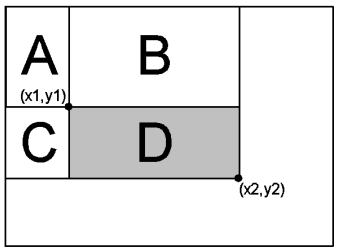
\includegraphics[width=0.7\linewidth]{./graphics/rectangle.png}
  \caption{Visualization of how integral image is used to calculate the sum over rectangle D} 
\end{figure}

\subsection{Efficient Preprocessing of Input Data}
\label{sub:sec:preprocessing}



\begin{itemize}
\item Reading many small files concurrently, with multiple threads (compared to a single thread), takes advantage of the internal parallelism of SSDs and thus leads to higher throughput \cite{Zhuang2016}.

\item C-string manipulation functions are often significantly faster than their C++ pendants. For example, locating substrings with \texttt{strstr} is around five times faster than using the C++ \texttt{std::string} function \texttt{find}.

\item Hardcoding regular expressions with \emph{while, for, switch} or \emph{if-else} statements results in faster execution times than using standard RegEx libraries, where regular expressions are compiled at runtime into state machines.

\item Changing strings in place, instead of treating them as immutable objects, eliminates allocation and copying overhead.

\end{itemize}


\section{Experiments}

Table~\ref{tab:results} shows the running times of the resolution step of the five best placed teams.


\begin{table}[htbp]
  \caption{Comparison of the F-measure and the running times of the resolution step of the five best placed teams. The input data for the resolution step consisted of 29{,}787 in JSON formatted e-commerce websites. Measurements were taken on a
laptop running Ubuntu 19.04 with 16 GB of RAM and two Intel Core i5-4310U CPUs. The underlying SSD was a 500\,GB 860 EVO mSATA. We cleared the page cache, dentries, and inodes before each run to avoid reading the input data from RAM instead of the SSD.}
  \label{tab:results}
\resizebox{\columnwidth}{!}{
  \begin{tabular}{lcrr}
    \toprule
    Team& Language & F-measure & Running time (s)\\
    \midrule
	PictureMe (\textbf{this paper}) &C++& 0.99 & \textbf{0.61}\\
    DBGroup@UniMoRe &Python& 0.99 & 10.65\\
    DBGroup@SUSTech &C++& 0.99 & 22.13\\
    eats\_shoots\_and\_leaves &Python& 0.99 & 28.66\\
    DBTHU &Python& 0.99& 63.21\\
  \bottomrule
\end{tabular}
}
\end{table}


\section{Conclusions}

%%
%% The next two lines define the bibliography style to be used, and
%% the bibliography file.
\begin{thebibliography}{h}
\bibitem{LecSource1}Bilal Bataineh, Siti N.H.S. Abdullah, K. Omar, M. Faidzul. Adaptive Thresholding Methods for Documents Image Binarization, Universiti Kebangsaan Malaysia,  Springer-Verlag Berlin Heidelberg, 2011
\bibitem{LecSource2}Derek Bradley, Gerhard Roth. Adaptive Thresholding Using the Integral Image, Journal of Graphics GPU and Game Tool, 2007
\bibitem{LecSource3}Bolan Su, Shijian Lu, Chew Lim Tan. Binarization of historical document images using the local maximum and minimum, DAS '10: Proceedings of the 9th IAPR International Workshop on Document Analysis Systems, 2010, Pages 159–166

\end{thebibliography}

\newpage

\section{still to be settled/focused on}

\begin{itemize}
    \item Paragraphing, maybe i should press enter more often
    
\end{itemize}

\end{document}
\endinput
%%
%% End of file `sample-sigconf.tex'.
